\subsection{局部紧空间}

定义 4. 拓扑空间 X 称为局部紧的，如果它是豪斯多夫的且 X 的每一点都有一个紧邻域。

显然紧空间是局部紧的，但反之不真；例如，每个离散空间都是局部紧的，但若是无限的则不是紧的。

* 我们将在第四章 § 2 中看到，实直线 R 是局部紧的，但不是紧的。*

命题 9. 每个局部紧空间都是正则的。

设 X 是局部紧空间，则每点 \(x \in X\) 都有一个紧邻域 V；既然 X 是豪斯多夫的，V 是闭的（第 3 目，命题 4）。另一方面，V 是 X 的正则子空间（第 2 目，命题 1 的推论），因此 X 是正则的（§ 8，第 4 目，命题 13）。

推论. 在局部紧空间中，每一点都有一个紧邻域组成的基本邻域系。

因为 x 的一个闭邻域与 x 的一个紧邻域之交是 x 的一个紧邻域（第 3 目，命题 3）。

\pandocbounded{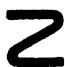
\includegraphics[keepaspectratio]{images/part001_13daf5c9.jpg}}

存在这样的非豪斯多夫拓扑空间，其中每一点都有一个由紧邻域组成的基本邻域系（习题 5）。

命题 9 的推论可以如下推广：

命题 10. 在局部紧空间 X 中，每个紧集 K 都有一个由紧邻域组成的基本邻域系。

设 \(\mathbf{U}\) 是 \(\mathbf{K}\) 的任一邻域。对每个 \(x \in \mathbf{K}\)，存在紧邻域 \(\mathbf{W}(x)\)（即 \(x\) 的紧邻域），它包含于 \(\mathbf{U}\)。当 x 跑遍 K 时，诸集合

W (x) 的内部构成 K 的一个开覆盖；于是存在有限多个点 \(x_{i} \in K\)（\(1 \leqslant i \leqslant n\)），使诸 \(W(x_{i})\) 的内部覆盖 K。因此诸 \(W(x_{i})\) 的并 V 是 K 的一个包含于 U 中的紧邻域（第 3 目，命题 5）。

命题 11. 设 X 是局部紧空间，F 是 X 的一个子集，使得每当 K 是 X 的紧子集时 \(F \cap K\) 都是紧的。则 F 在 X 中是闭的。

鉴于第 3 目命题 4，这由 § 3 第 1 目命题 3 a) 得出。

命题 12. 在豪斯多夫空间 X 中，每个局部紧子空间 A 都是局部闭的。

由假设，对每个 \(x \in A\)，存在 x 在 X 中的一个邻域 V，使得 \(V \cap A\) 是紧的，从而在 V 中是闭的（第 3 目，命题 4）。

命题 13. 局部紧空间 X 的每个局部闭子空间都是局部紧的。

设 A 是 X 的一个局部闭子空间；则对每个 \(x \in A\)，存在 x 在 X 中的一个邻域 U，使得 \(U \cap A\) 在 U 中是闭的。设 \(V \subset U\) 是 x 在 X 中的一个紧邻域；\(V \cap A = V \cap (U \cap A)\) 在 V 中是闭的，从而是紧的（第 3 目，命题 3）。既然 \(V \cap A\) 是 x 在 A 中的一个邻域，结论得证（显然 A 是豪斯多夫的）。

\pandocbounded{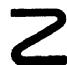
\includegraphics[keepaspectratio]{images/part001_5df2d3a1.jpg}}

定理 1（第 1 目）与定理 2 的推论 2（第 4 目）不能推广到非紧的局部紧空间。

例如，在无限离散空间 X 中，由包含给定点 \(x \in X\) 且余集有限的那些集合组成的滤子以 x 为唯一聚点，但不收敛于 x。既然 X 到豪斯多夫空间 \(X'\) 中的任何映射 f 都连续，f 之下 X 的任一子集（因 X 是离散的，它在 X 中是闭的）的象一般不是 \(X'\) 的闭子集。

与第 5 目定理 3 相应的命题如下：

命题 14. a) 设 \((\mathbf{X}_{\iota})_{\iota \in I}\) 是局部紧空间的一个族，使得除有限多个指标外 \(\mathbf{X}_{\iota}\) 都是紧的。则积空间 \(\mathbf{X} = \prod_{\iota \in I} \mathbf{X}_{\iota}\) 是局部紧的。

\begin{enumerate}
\def\labelenumi{\alph{enumi})}
\setcounter{enumi}{1}
\item
  反之，若非空拓扑空间的族 \((\mathbf{X}_{\iota})_{\iota\in I}\) 的积是局部紧的，则除有限多个指标外诸因子 \(\mathbf{X}_{\iota}\) 都是紧的，且不紧的那些因子是局部紧的。
\item
  设 \(x = (x_{\iota})\) 是 \(X\) 的一点。对每个指标 \(\iota \in I\)，若 \(X_{\iota}\) 局部紧但不紧，则设 \(V_{\iota}\) 是 \(x_{\iota}\) 在 \(X_{\iota}\) 中的一个紧邻域，而对所有其他指标 \(\iota\) 令 \(V_{\iota} = X_{\iota}\)。则 \(\prod_{\iota \in I} V_{\iota}\) 是 \(x\) 在 \(X\) 中的一个紧邻域（第 5 目，定理 3）。又由 § 8 第 2 目命题 7，\(X\) 是豪斯多夫的，从而是局部紧的。
\item
  若 \(X = \prod_{\iota \in I} X_{\iota}\) 是局部紧的且诸 \(X_{\iota}\) 非空，则每个 \(X_{\iota}\) 同胚于 \(X\) 的一个闭子空间（§ 4，第 2 目，命题 4 及 § 4，第 3 目，命题 7 的推论），于是由命题 13 是局部紧的。设 \(a = (a_{\iota})\) 是 \(X\) 的一点，\(V\) 是 \(a\) 的一个紧邻域；既然除有限多个指标外我们有 \(pr_{\iota}V = X_{\iota}\)（§ 4，第 1 目），则由第 4 目定理 2 的推论 1，除有限多个指标外诸 \(X_{\iota}\) 都是紧的。
\end{enumerate}

